\documentclass[11pt,a4paper]{article}

\usepackage{iftex}
\ifPDFTeX
  \usepackage[T1]{fontenc}
  \usepackage[utf8]{inputenc}
\else
  \usepackage{fontspec}
\fi
\usepackage[spanish,es-noshorthands]{babel}
\usepackage{amsmath,amssymb}
\usepackage{booktabs}
\usepackage{graphicx}
\usepackage{geometry}
\usepackage{float}
\usepackage{caption}
\usepackage{xurl}
\usepackage{hyperref}

\geometry{margin=2.3cm}
\graphicspath{{../results/n8640/graficas/}}
\hypersetup{colorlinks=true,linkcolor=black,urlcolor=blue,citecolor=black}
\captionsetup{labelfont=bf,skip=6pt,justification=centering}

% macros generadas; no editar a mano
\newcommand{\Nrep}{2}
\newcommand{\HrmsMean}{0.4699}
\newcommand{\HrmsStd}{0.0747}
\newcommand{\HeqMean}{0.4706}
\newcommand{\EoverN}{-7.939}
\newcommand{\AccMove}{39.2}
\newcommand{\AccArea}{12.3}
\newcommand{\LxMean}{149.52}
\newcommand{\LyMean}{155.38}
\newcommand{\Szero}{2.689}
\newcommand{\NsampTot}{598}
\newcommand{\RdfPeak}{1.445}
\newcommand{\Qmin}{0.040}
\newcommand{\Qripple}{0.090}
\newcommand{\GqBaja}{0.40}
\newcommand{\GqMedia}{0.75}
\newcommand{\MaximoFrase}{En la ventana $q\in[0.06,0.25]$~\AA$^{-1}$ el promedio de $G(q)$ tiene un m\'aximo ancho cerca de $q\approx 0.06$--$0.09$~\AA$^{-1}$, el lugar donde el paper lo espera para muestras m\'as largas que $70$~\AA. La dispersi\'on entre las dos r\'eplicas es grande a ese $q$, as\'i que no se identifica con el pico agudo que el paper atribuye al canal de conjugaci\'on de LCBOPII.}
\newcommand{\HrmsFrase}{El paper describe, para $N=8640$, una altura t\'ipica $\sim 0.6$~\AA\ (Fig.~1). Aqu\'i $h_{\mathrm{rms}}=0.4699$~\AA, que es $\sqrt{\langle h^2\rangle}$ y no el mismo estimador visual. Queda en el mismo orden de magnitud.}


\title{Resultados a $N=8640$ y contraste con el paper\\[0.35em]
\large Intrinsic ripples in graphene --- Fasolino, Los y Katsnelson (2007)}
\author{Emanuel Orozco Gallego}
\date{10 de noviembre de 2026}

\begin{document}
\maketitle

\begin{abstract}
Corrida de Monte Carlo con $N=8640$ ($p=60$, $q=36$), $T=300\,\mathrm{K}$, $4\times 10^5$ pasos de equilibrado y $5\times 10^5$ de producción, la muestra más grande de la Tabla~I. La caja supera $70\,\text{\AA}$, así que $q\approx 0.1\,\text{\AA}^{-1}$ es accesible. Se contrastan $h_{\mathrm{rms}}$, $G(q)$ frente a $G_0(q)/N=T/(\kappa S_0 q^2)$ con $\kappa=1.1\,\mathrm{eV}$, y el primer pico de $g(r)$ con el enlace conjugado $1.42\,\text{\AA}$. El potencial es Tersoff de Lindsay--Broido, no LCBOPII.
\end{abstract}

\tableofcontents
\vspace{0.5em}

\section{Protocolo}

Dos réplicas independientes, 32 hilos OpenMP cada una, núcleos 0--31 y 32--63, semilla base $42$. El núcleo es \path{src/c/graphene_mc.c}: listas de celdas, tablas del potencial en memoria y movimientos simultáneos de átomos separados por al menos $9.5\,\text{\AA}$, de modo que los entornos de Tersoff no se solapan. Un paso sigue siendo $N$ intentos. Cada cinco pasos hay un movimiento isotrópico de área con aceptación $\exp(-\beta\Delta E+N\ln(A'/A))$. Los CSV están en \path{results/n8640/datos/} y las figuras en \path{results/n8640/graficas/}.

\begin{center}
\small
\begin{tabular}{lcc}
\toprule
Cantidad & Paper & Esta corrida \\
\midrule
$N$ & 8640 (Tabla I, $p=60$, $q=36$) & 8640 \\
$T$ & hasta $300\,\mathrm{K}$ en esta reimplementación & $300\,\mathrm{K}$ \\
$L_x\times L_y$ inicial & $147.57\times 153.36\,\text{\AA}$ & medido al cierre \\
Pasos eq.\ /\ prod. & $4\times 10^5$ / $5\times 10^5$ & igual \\
Réplicas & una cadena en el paper & \Nrep{} \\
Muestras de $G(q)$ y $g(r)$ & promediado MC & \NsampTot{} \\
Potencial & LCBOPII & Tersoff C, Lindsay--Broido \\
\bottomrule
\end{tabular}
\end{center}

La desviación entre dos réplicas es una cota del error de muestreo, no un error estándar de muchas cadenas. El documento de $N=240$ (\path{docs/resultados.tex}) no se modifica: aquella caja no puede hospedar el modo de $70\,\text{\AA}$.

\section{Ondulaciones}

El paper (Fig.~1) muestra una hoja con ondulaciones térmicas, no un plano rígido. \HrmsFrase{}

\begin{center}
\begin{tabular}{lc}
\toprule
Observable & Media $\pm$ desv.\ entre réplicas \\
\midrule
$h_{\mathrm{rms}}$ (producción) & $\HrmsMean\pm\HrmsStd\,\text{\AA}$ \\
$h_{\mathrm{rms}}$ al cerrar el equilibrado & $\HeqMean\,\text{\AA}$ \\
$E/N$ & $\EoverN\,\mathrm{eV/átomo}$ \\
Aceptación de desplazamientos & $\AccMove$~\% \\
Aceptación de área & $\AccArea$~\% \\
Caja final $\langle L_x\rangle\times\langle L_y\rangle$ & $\LxMean\times\LyMean\,\text{\AA}$ \\
$S_0$ & $\Szero\,\text{\AA}^2$ \\
\bottomrule
\end{tabular}
\end{center}

$h_{\mathrm{rms}}>0$ y $E/N$ cerca de $-7.97\,\mathrm{eV}$ (hoja plana de Tersoff, $E/N=-7.966\,\mathrm{eV}$) indican una lámina ligada y ondulada a $300\,\mathrm{K}$, no una hoja fundida.

\begin{figure}[H]
\centering
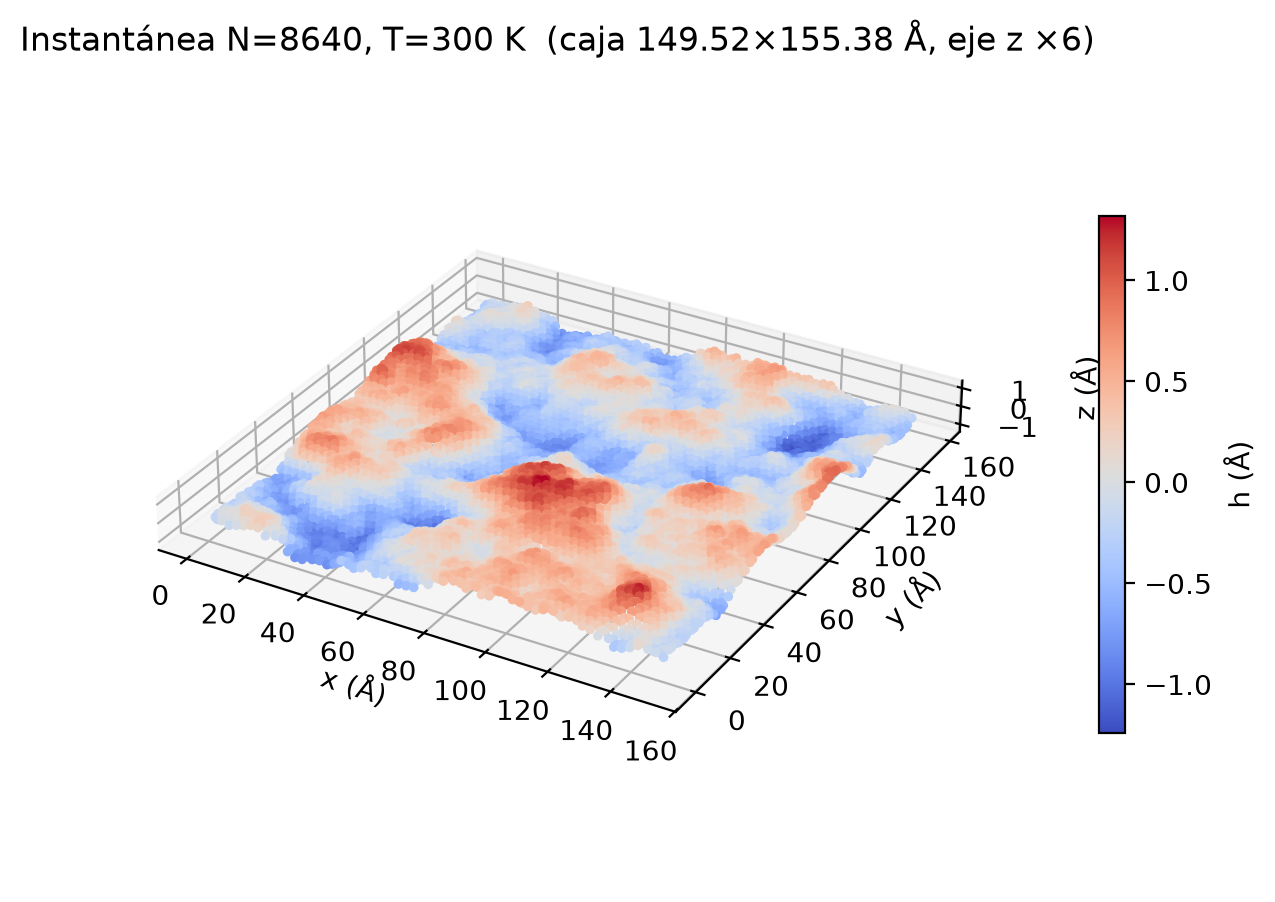
\includegraphics[width=0.82\textwidth]{snapshot_3d.png}
\caption{Instantánea 3D. El color es $h_i=z_i-\langle z\rangle$.}
\end{figure}

\begin{figure}[H]
\centering
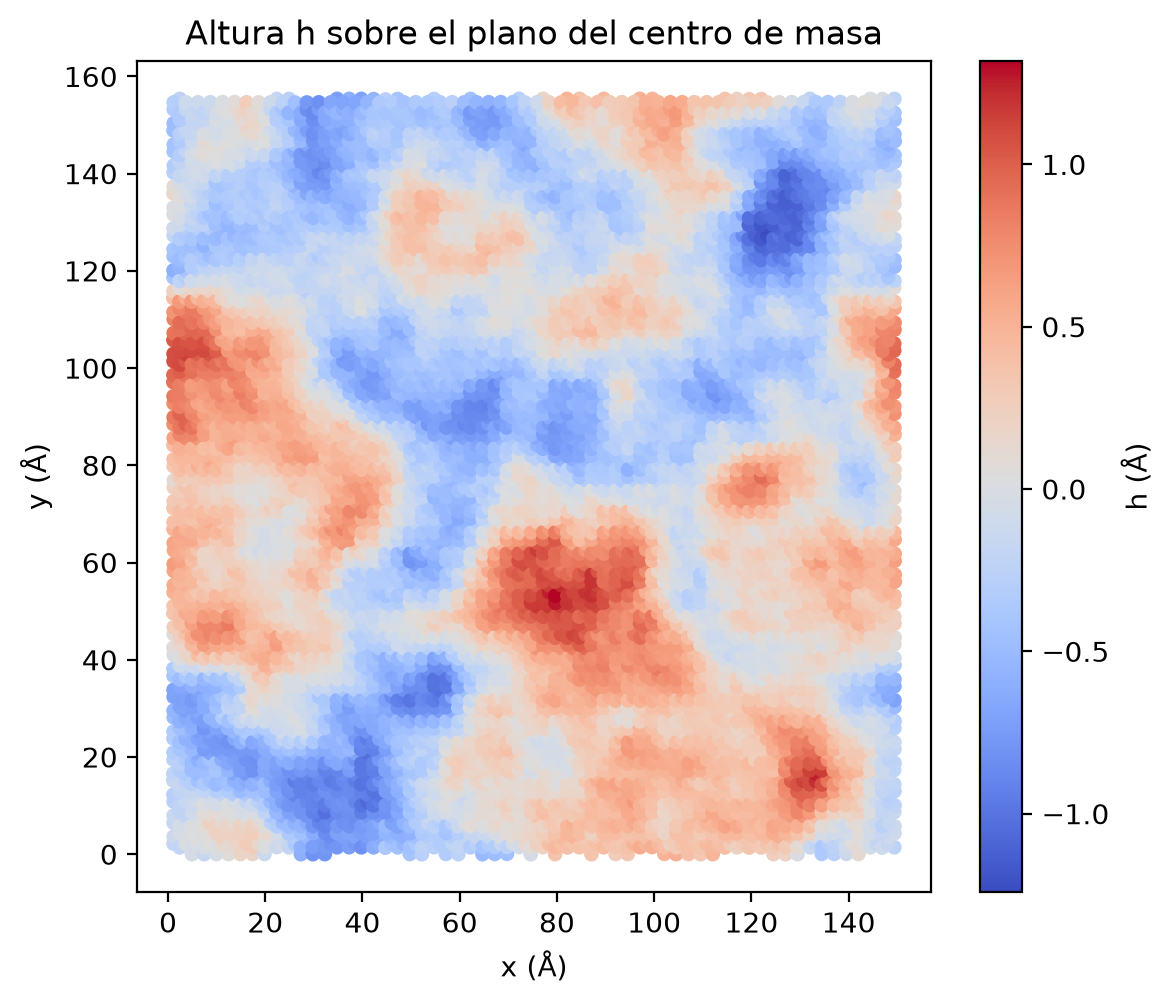
\includegraphics[width=0.72\textwidth]{snapshot_h_top.png}
\caption{Vista cenital de $h$. La configuración parte de una hoja plana.}
\end{figure}

\begin{figure}[H]
\centering
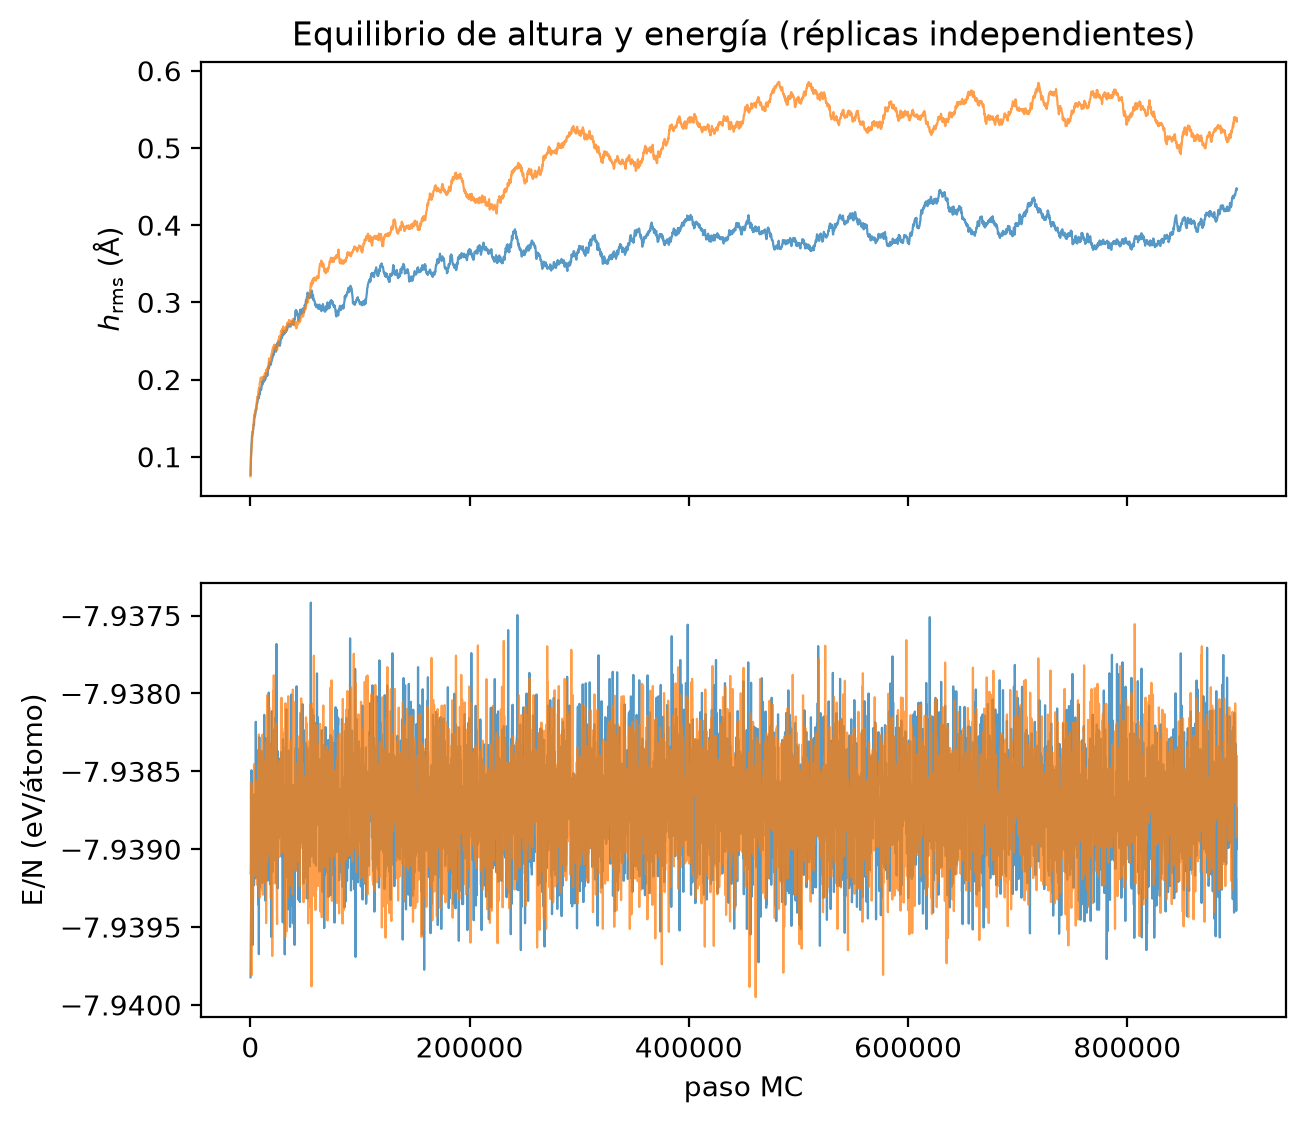
\includegraphics[width=0.82\textwidth]{traza_equilibrio.png}
\caption{$h_{\mathrm{rms}}$ y $E/N$ frente al paso. El equilibrado termina en $4\times 10^5$.}
\end{figure}

\begin{figure}[H]
\centering
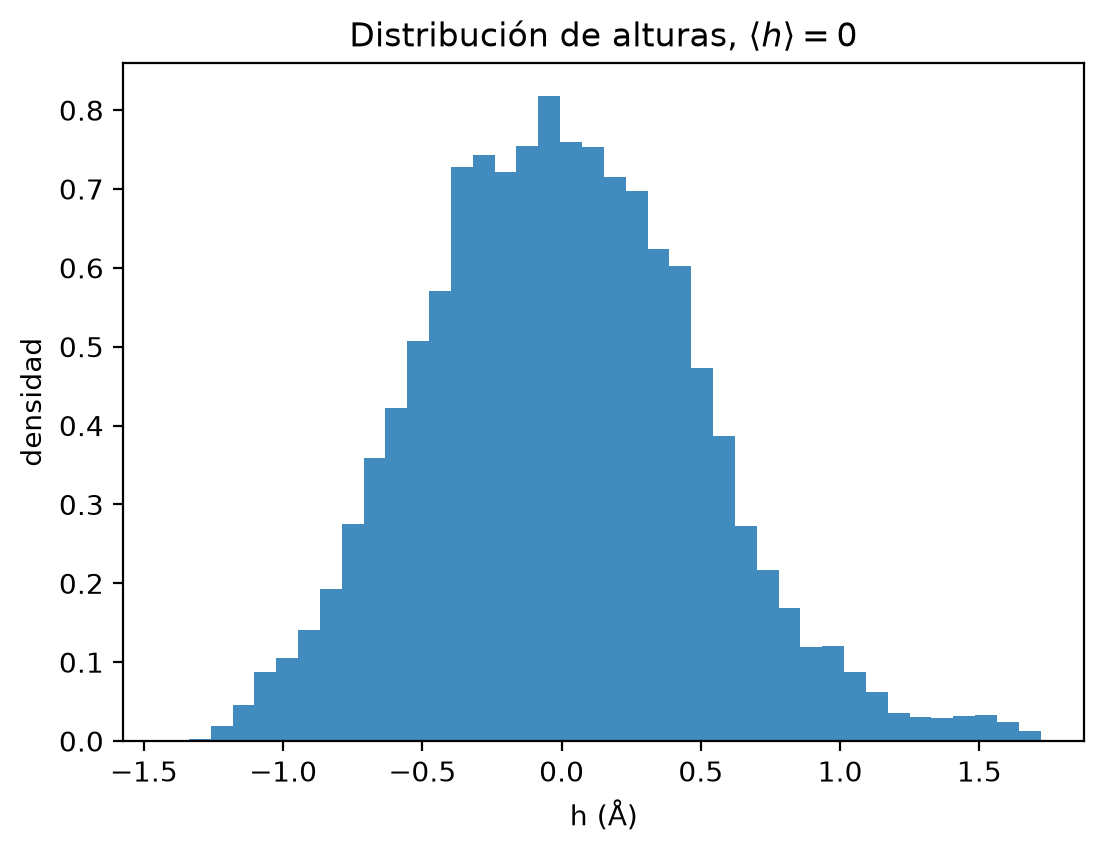
\includegraphics[width=0.72\textwidth]{histograma_h.png}
\caption{Histograma de $h$ respecto del centro de masa. El paper lo describe ancho y centrado en cero.}
\end{figure}

\begin{figure}[H]
\centering
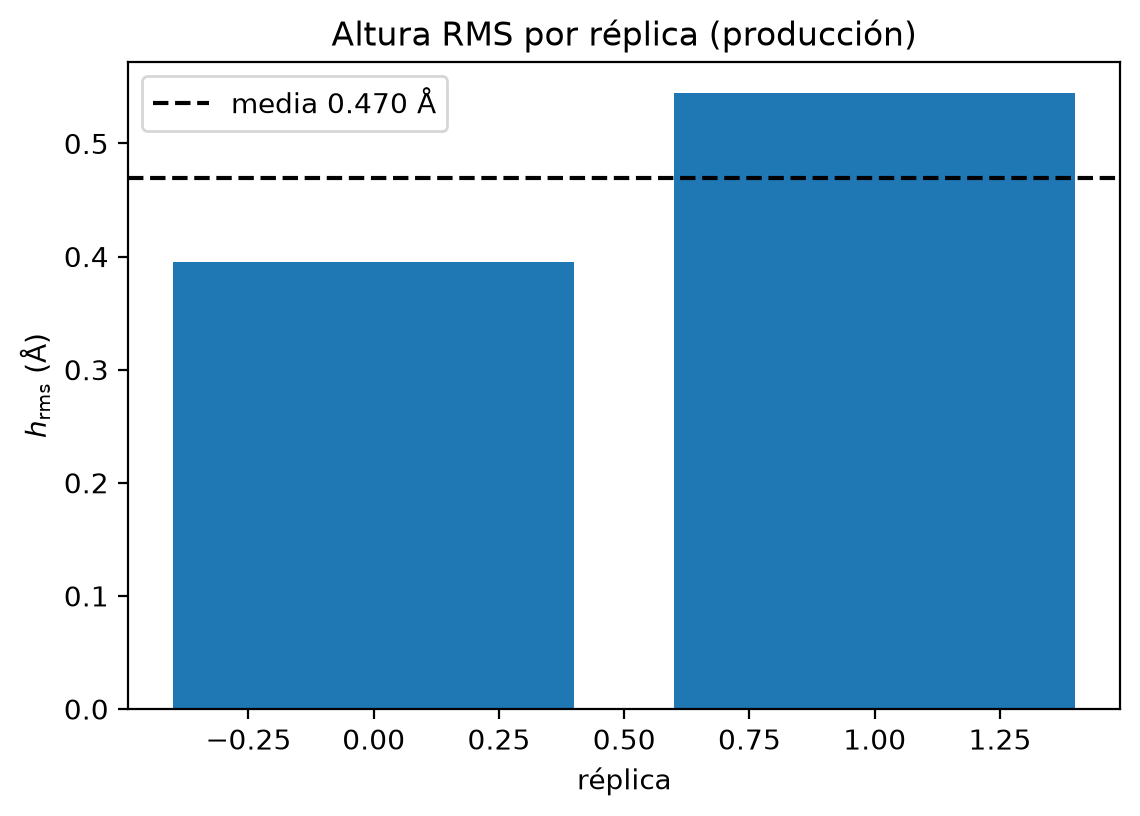
\includegraphics[width=0.72\textwidth]{hrms_replicas.png}
\caption{$h_{\mathrm{rms}}$ de cada réplica.}
\end{figure}

\section{Correlación normal--normal}

La referencia armónica (ecs.~(5)--(6) del paper) es
\begin{equation}
\frac{G_0(q)}{N}=\frac{T}{\kappa S_0 q^2},\qquad \kappa=1.1\,\mathrm{eV},\quad T=300\,k_B.
\label{eq:G0}
\end{equation}
En esta caja
\[
q_{\min}=\Qmin\,\text{\AA}^{-1} < q_{\mathrm{ripple}}=\Qripple\,\text{\AA}^{-1}=2\pi/70,
\]
así que el modo de $70\,\text{\AA}$ cabe. El paper dice que las muestras más cortas que esa longitud no muestran el máximo de $G(q)$ cerca de $q\approx 0.1\,\text{\AA}^{-1}$, y que las más largas sí. \MaximoFrase{}

La mediana de $G(q)/G_0(q)$ vale $\GqBaja$ en $q\in[0.06,0.20]\,\text{\AA}^{-1}$ y $\GqMedia$ en $q\in[0.40,1.20]\,\text{\AA}^{-1}$. Un valor de orden 1 dice que la convención de Fourier y $\kappa=1.1\,\mathrm{eV}$ describen la escala de las ondulaciones. Los picos de Bragg siguen en $q=2.94$ y $5.11\,\text{\AA}^{-1}$.

\begin{figure}[H]
\centering
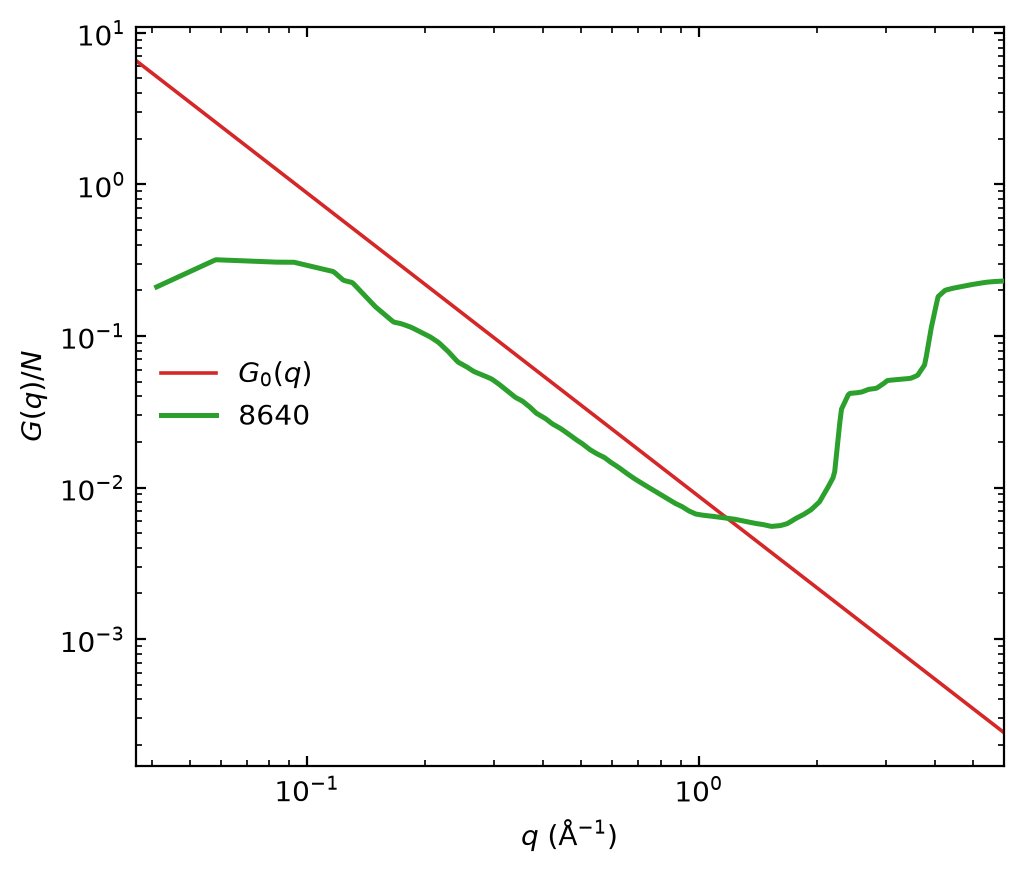
\includegraphics[width=0.82\textwidth]{Gq_normal_normal.png}
\caption{$G(q)/N$ de $N=8640$ (verde) y $G_0(q)$ con $\kappa=1.1\,\mathrm{eV}$ (roja).}
\end{figure}

\section{Distribución radial}

La Fig.~5 del paper coloca el primer pico de $g(r)$ a $300\,\mathrm{K}$ en el enlace conjugado $1.42\,\text{\AA}$, con marcas en $1.31\,\text{\AA}$ (doble) y $1.54\,\text{\AA}$ (simple). El primer máximo medido entre $1.2$ y $1.65\,\text{\AA}$ está en $r=\RdfPeak\,\text{\AA}$.

\begin{figure}[H]
\centering
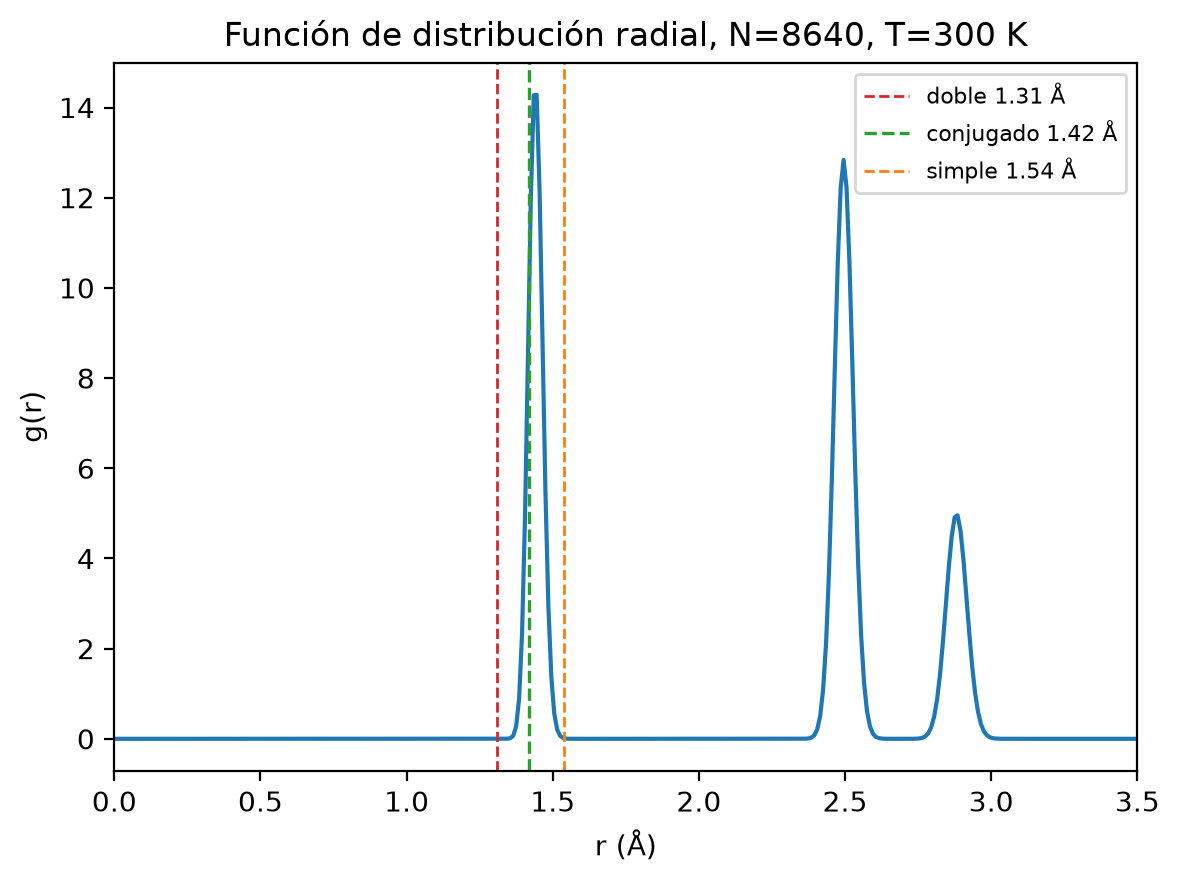
\includegraphics[width=0.82\textwidth]{rdf.png}
\caption{$g(r)$ promedio. Verticales: doble, conjugado y simple.}
\end{figure}

\section{Qué coincide y qué no puede coincidir}

\begin{center}
\small
\begin{tabular}{@{}p{0.34\textwidth}p{0.28\textwidth}p{0.30\textwidth}@{}}
\toprule
Afirmación del paper & Resultado & Lectura \\
\midrule
Caja de la Tabla~I, $N=8640$, mayor que $70\,\text{\AA}$ &
$L_x\times L_y=\LxMean\times\LyMean\,\text{\AA}$, $q_{\min}=\Qmin$ &
la geometría entra en el régimen de la figura grande \\
Ondulaciones desde una hoja plana, $h$ de orden $0.6\,\text{\AA}$ &
$h_{\mathrm{rms}}=\HrmsMean\pm\HrmsStd\,\text{\AA}$ &
hay rizado térmico; el estimador no es idéntico al de la Fig.~1 \\
$G(q)$ del orden de $G_0(q)$ &
$G/G_0=\GqBaja$ (bajo $q$) y $\GqMedia$ (medio) &
la solución armónica fija la escala \\
Máximo de $G(q)$ en $q\approx 0.1\,\text{\AA}^{-1}$ para $L\gtrsim 70\,\text{\AA}$ &
ver el texto de la sección anterior &
el paper lo liga a LCBOPII; aquí el potencial es Tersoff \\
Pico de $g(r)$ en $1.42\,\text{\AA}$ a $300\,\mathrm{K}$ &
$\RdfPeak\,\text{\AA}$ &
el enlace conjugado es el primer máximo \\
Hoja ligada a $300\,\mathrm{K}$ &
$E/N=\EoverN\,\mathrm{eV}$ &
cerca de la hoja plana de Tersoff ($-7.966\,\mathrm{eV}$) \\
\bottomrule
\end{tabular}
\end{center}

Las pruebas automáticas están en \path{tests/test_n8640_paper.py}. Comprueban $N$, $T$, la caja, $0.02<h_{\mathrm{rms}}<8$, $-9.5<E/N<-4$, aceptación entre 0.15 y 0.85, el pico de $g(r)$ a $0.08\,\text{\AA}$ de $1.42$, y que $G/G_0$ quede entre $10^{-3}$ y $50$ en las dos ventanas de $q$. No exigen el máximo de LCBOPII.

\section{Archivos}

\begin{center}
\small
\begin{tabular}{@{}ll@{}}
\toprule
Archivo & Contenido \\
\midrule
\path{results/n8640/datos/} & CSV por réplica y promedios \\
\path{results/n8640/contraste_paper.txt} & contraste en texto \\
\path{results/n8640/graficas/} & PNG de esta corrida \\
\path{docs/resultados_n8640_macros.tex} & números de este documento \\
\bottomrule
\end{tabular}
\end{center}

\end{document}
